\documentclass[a4paper,10pt]{article}
\usepackage[utf8]{inputenc}
\usepackage{amsfonts}
\usepackage{amssymb}
\usepackage{amsmath}
\usepackage{mathrsfs}
\usepackage{amsbsy}
\usepackage{ragged2e}
\usepackage{graphicx}
\usepackage[verbose]{wrapfig}
\usepackage{changepage}
\usepackage{float}
\usepackage{cite}
\usepackage{url}
\usepackage{geometry}                         
\geometry{left=18mm,right=18mm,top=21mm,bottom=21mm}
\usepackage[usenames,dvipsnames]{xcolor}
\pagecolor{white}
\usepackage{multirow}
\definecolor{wiki}{rgb}{1,0.5,0}
\usepackage{tikz}
\usepackage{array}
\usepackage[all]{xy}
\usepackage{tabularx}
\usepackage{subcaption}
\graphicspath{Images}
\pagestyle{plain} 
\pagenumbering{arabic}
\usepackage{lastpage}
\usepackage{fancyhdr}
\pagestyle{fancy}
\usepackage{lipsum}
\usepackage{booktabs}
\usepackage{skull}
\usepackage{multicol}
\usepackage{parcolumns}
\usepackage{soul}
\usepackage[hidelinks]{hyperref} 


\definecolor{MiColor1}{RGB}{135,2,1}
\definecolor{MiColor2}{RGB}{254,80,0}
\definecolor{MiColor3}{RGB}{44,135,240}
\definecolor{MiColor4}{RGB}{6,69,173}
\definecolor{MiColor5}{RGB}{51,102,187}

\lhead{\protect\href{https://www.uaeh.edu.mx/}{
\includegraphics[width=.12\textwidth]{Images/UAEH Logo.png}}} 
\chead{\itshape{August 2020}}
\rhead{\colorbox{MiColor1}{\textcolor{White}{\protect\href{https://www.uaeh.edu.mx/campus/icbi/oferta/licenciaturas/lic_fisica.html}{LiFTA}}}} 
\lfoot{} 
\cfoot{\thepage\ of \pageref{LastPage}} 
\rfoot{}


\renewcommand{\headrulewidth}{2pt}
\renewcommand{\footrulewidth}{0pt}


\setlength\headheight{55.0pt}
\addtolength{\textheight}{-40.0pt}
%-------------------------------%

\newcounter{resumen}
\setcounter{resumen}{0}
\def\theejemplo{\thechapter.\arabic{resumen}}

\newenvironment{resumen}
{	\begin{center}
	\begin{minipage}[t!]{480 pt}
	\vspace{2mm}
	\emph{\textcolor{MiColor1}{\textbf{Abstract}}}
	\\[-1mm]
	\\[-10mm]
	\hfill 
	   \begin{wrapfigure}{hbt!}{6.8cm}
       \centering
       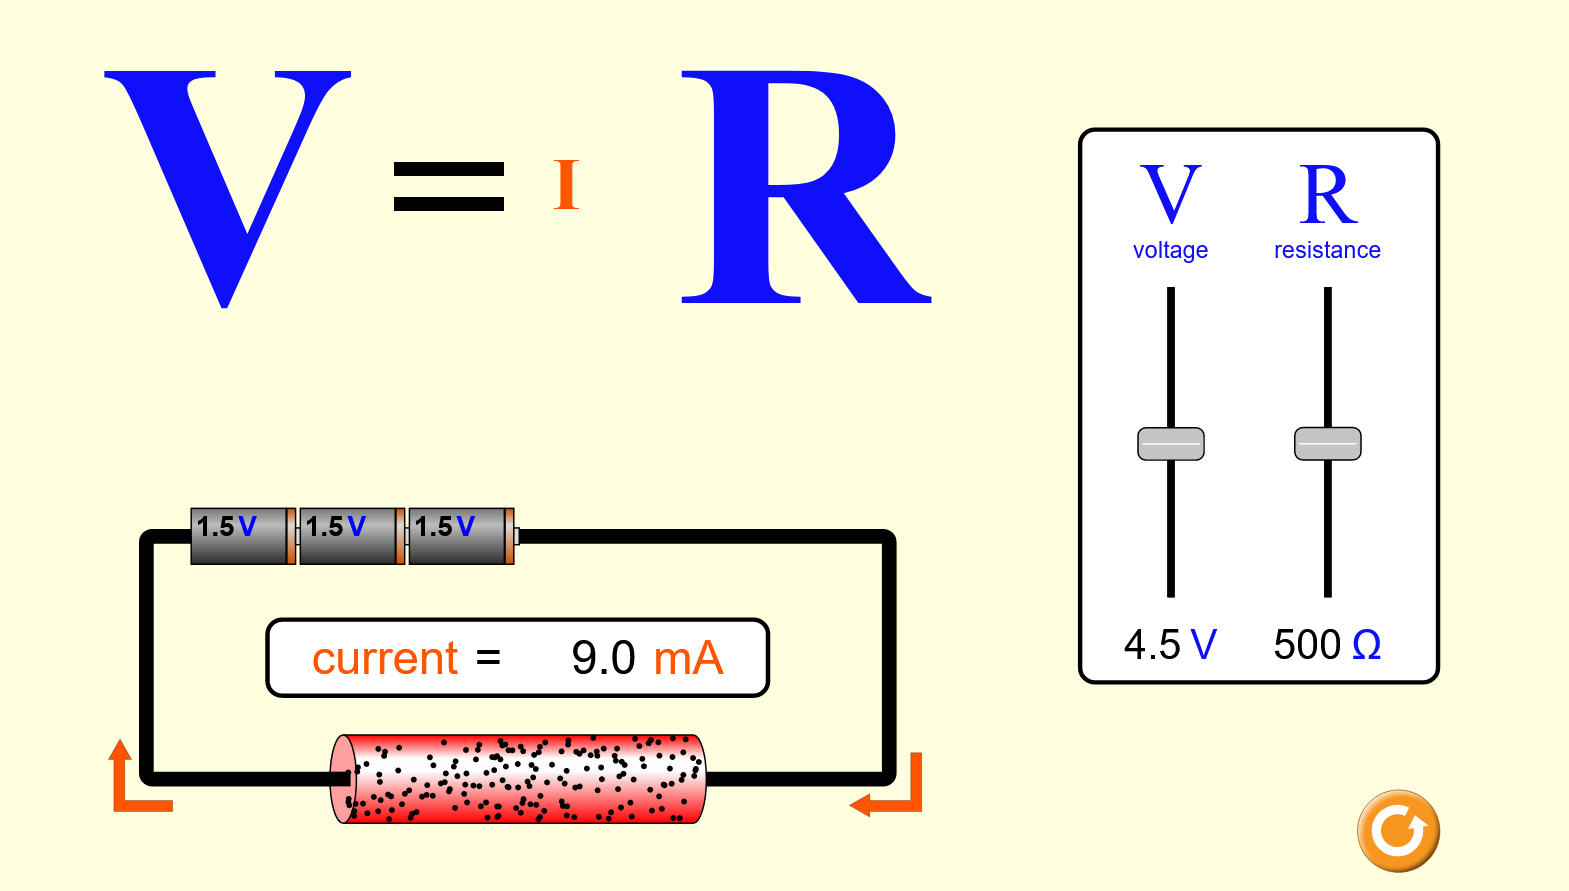
\includegraphics[scale=0.2]{Images/Ohm's Law.PNG}
       \end{wrapfigure} \vspace{-4.8mm}
    \hfill
	\textcolor{Black}{\line(1,0){480}}\\ \par
}
{
	\par \normalsize \par
	\par \\[3mm] \par
	\vspace{4mm}
	\par \footnotesize\textbf{Keywords: \footnotesize\@palabras}
	\\[-1mm]
	\textcolor{Black}{\line(1,0){480}}\\ \par
	\\[5cm]
	\end{minipage}
	\vspace{0.5cm}
	\end{center}
}


\def\palabras#1{\gdef\@palabras{#1}}

\palabras{Electric current, Resistance, Voltage, Ohm$'$s law, Changing values and Independent values} 

%-------------------------------%

\begin{document}

{\textbf{\LARGE Ohm's Law} \par} \vspace{3mm}
{\small A. D. Hernández-Melo\textcolor{Plum}{$^\heartsuit$}, E. S. Pulido-Reyes\textcolor{ProcessBlue}{$^\diamondsuit$}, y A. A. Santoyo-Noeggerath\textcolor{Green}{$^\dagger$} \par} \vspace{3mm}
{\footnotesize \textcolor{Plum}{$^\heartsuit$}\textcolor{ProcessBlue}{$^\diamondsuit$}\textcolor{Green}{$^\dagger$}\protect\href{https://www.google.com/maps/place/\%C3\%81rea+Acad\%C3\%A9mica+de+Matem\%C3\%A1ticas+y+F\%C3\%ADsica,+Universidad+Aut\%C3\%B3noma+del+Estado+de+Hidalgo,+Universidad+Autonoma+del+Estado+de+Hidalgo/@20.0934375,-98.7104375,17z/data=!4m13!1m7!3m6!1s0x0:0x0!2s76G337VQ\%2B9R!3b1!8m2!3d20.0934375!4d-98.7104375!3m4!1s0x85d1a773691bc455:0xe552799fa3ca76a5!8m2!3d20.0933901!4d-98.7104677}{Área Académica de Matemáticas y Física, Instituto de Ciencias Básicas e Ingenierías, Universidad Autónoma del Estado} \par} 
{\footnotesize \protect\href{https://www.google.com/maps/place/\%C3\%81rea+Acad\%C3\%A9mica+de+Matem\%C3\%A1ticas+y+F\%C3\%ADsica,+Universidad+Aut\%C3\%B3noma+del+Estado+de+Hidalgo,+Universidad+Autonoma+del+Estado+de+Hidalgo/@20.0934375,-98.7104375,17z/data=!4m13!1m7!3m6!1s0x0:0x0!2s76G337VQ\%2B9R!3b1!8m2!3d20.0934375!4d-98.7104375!3m4!1s0x85d1a773691bc455:0xe552799fa3ca76a5!8m2!3d20.0933901!4d-98.7104677}{de Hidalgo, Carretera Pachuca-Tulancingo Km. 4.5, Col. Carboneras, C.P. 42184, Mineral de la Reforma, Hidalgo, México} \par}
{\footnotesize \textit{Contact}: \textcolor{Plum}{$^\heartsuit$}\protect\href{mailto:he312453@uaeh.edu.mx}{he312453@uaeh.edu.mx},  \textcolor{ProcessBlue}{$^\diamondsuit$}\protect\href{mailto:pu359528@uaeh.edu.mx}{pu359528@uaeh.edu.mx}, \textcolor{Green}{$^\dagger$}\protect\href{mailto:sa352740@uaeh.edu.mx}{sa352740@uaeh.edu.mx}}

\begin{resumen}
The electrical circuits knowledge and their utility nowadays it's fundamental to a "day to day" routine, practically almost all the items or things the we use needs electric energy to work on: a cellphone, the computer, a microwave, and so on; and part of the way that this items obtain electric energy it's and electric circuit and part of the components of and electric circuit it's what are on the Ohm's law, over this practice's report it going to be possible have a better comprehension about three components that are fundamental to an electrical circuit.
Supporting this practice on the \textit{PhET} Software it going to be possible to watch and appreciate how the three components of the Ohm's Law: resistance, voltage and electric current keep some relation each other and watch what happen when there are values in constant movement or when there are not, and from this manner the graphs and physics relations (or "mathematical formulas") that going to be on the next sections explain how this law works, explaining the graphs comportment and some reasons of why are so important nowadays. This work also works like an experimental substance to the topics that were seen in the course of electromagnetism.
\end{resumen}

\begin{multicols}{2}
\section{\textcolor{MiColor1}{\textbf{Introduction}}}
The purpose of this paper was the study and understanding of Ohm's Law, analyzing its components (resistance, voltage and electric current) at an experimental way. Ohm's Law states that in a lot of materials (even in the majority of metals) the relation of the current density to electric field its a constant $\sigma$ that is independent of electric field produced by the electric current. (R. Serway, J. Jewett. 2009)\cite{1}. \par
\vspace{2mm}
\centerline{$J=\dfrac{I}{A}$}
\vspace{2mm}
The last mathematical expression refers to the current density that is equal to the electric current per unit cross sectional area of a conductor. but also we must define the electrical resistivity ($\rho$) too, that it keeps constant when the Ohm's law satisfy the relation between the electric field and the current density: \par
\vspace{2mm}
\centerline{$\Vec{E}=\rho \Vec{J}$}
\vspace{2mm}
Also, the resistivity ($\rho$) is the reciprocal of the conductivity ($\sigma$), $\rho =\dfrac{1}{\sigma}$, \hspace{0.2em} so, we could express the electrical resistance or the electrical conductance as: \par
\vspace{2mm}
\centerline{$R=\rho \dfrac{\ell}{A}\hspace{1em};\hspace{1em}C=\sigma \dfrac{A}{\ell}$}
\vspace{2mm}
(Where $\ell$ is the length of the conductor) The resistance of a given object depends primarily on two factors: What material it is made of, and its shape. For a given material, the resistance is inversely proportional to the cross-sectional area. \cite{8} \\
At this point we need the term of voltage, in other words the electrical potential that usually we could describe it as $V=\dfrac{U}{q}$. That's the simplest way to describe it and in the case of this paper, we only used this way. \par
So, the equation that "describes" the Ohm's Law is: \par
\vspace{2mm}
\centerline{V=IR}
\vspace{2mm}
It's important to say that this equation define the resistance $R$ for any conductor, even if the Ohm's Law is fulfilled or not, only its correct to say it if $R$ is constant. (H. D. Young, R. A. Freedman. 2013) \cite{2}. \par
In fact, there's a Ohm's Law Wheel, that defines the relationship between the components from the Ohm's Law and the Joule's Law ($P=VI$ where $P$ is power, measured in watts) and could be really useful when you try to solve some problems. \par
Anyway, with the web extension \textit{Phet} (developed by the University of Colorado Boulder) we did a few simulations, where we've seen in an easy way how the Ohm's Law works.\par \vfill
\begin{center}
    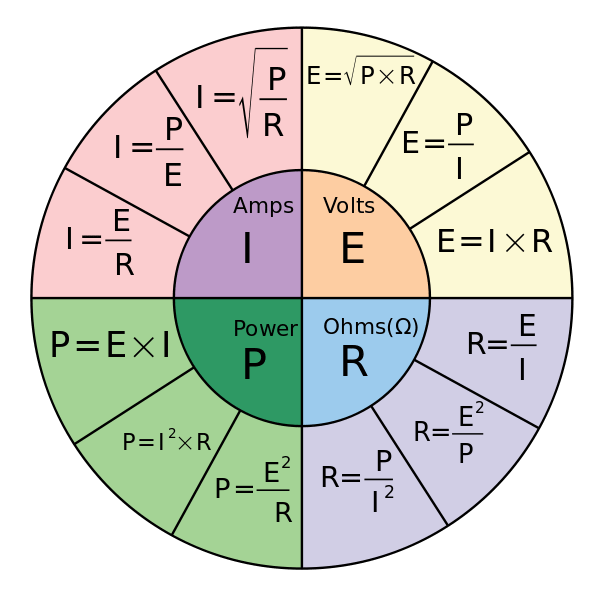
\includegraphics[scale=0.3]{Images/Ohms-Law-Formula-Wheel.png} \par
    \textcolor{MiColor2}{\textbf{Ohm's Law Wheel}}
\end{center}
\section{\textcolor{MiColor1}{\textbf{Materials and Experimental Methods}}}

\begin{table}[H]
    \centering
    \begin{tabular}{||>{\centering\arraybackslash}m{3.5cm} |>{\centering\arraybackslash}m{3.5cm}||}
    \hline
       \multirow{2}{3.5cm}{\centering\textbf{Description}} & \multirow{2}{3.5cm}{\centering\textbf{Specifications}} \\
        &  \\
    \hline \hline
       \multirow{3}{3.5cm}{\centering Conventional Computer} & \multirow{3}{3.5cm}{\centering Internet Connection} \\
        &  \\
        &  \\
    \hline
       \multirow{4}{3.5cm}{\centering Computer Software} & \multirow{4}{3.5cm}{\centering Web Extension \textit{PhET: Interactive Simulations}\cite{4}} \\
        &  \\
        &  \\
        &  \\
    \hline
       \multirow{2}{3.5cm}{\centering Computer Software} & \multirow{2}{3.5cm}{\centering OriginPro 2019} \\
        &  \\
    \hline
    \end{tabular}
\end{table}
\vspace{-3mm}
\begin{center}
    \textbf{Materials Table}
\end{center}
\vspace{-3mm}
\subsection{\textcolor{MiColor1}{\textbf{Experimental Methods}}}
In the \textit{PhET} simulator as the Graphical Abstract shows there are two variables that can be modified: voltage and resistance, the third: electric current cannot be modified, but this last one depends the other two so there proceed to modified voltage and resistance and watch the comportment of the system (as can be watch in the graphs), so there going to be three graphs, one where in the system the two independent values are in constantly change, in this case you can watch the values that the voltage and resistance take and how the electric current behalves; other where just the resistance changes, in this case the voltage going to be static, just taking one value for all the measurements, this value going to be five volts ($5V$) and the resistance is changing adding almost a hundred ohms ($100 \Omega$) every measurements; and other where just the voltage changes, in this last one the resistance stays static, taking a valor of three hundred three ohms ($303 \Omega$) and the voltage is constantly changing, adding one volt ($1V$) every measurement; at this way it can be possible to watch what happen with the electric current in the three cases proposed before and explain how the ohm's law works and the relations that it propose between resistance, voltage and electric current.
\section{\textcolor{MiColor1}{\textbf{Results}}}
\vspace{2em}
\begin{center}
      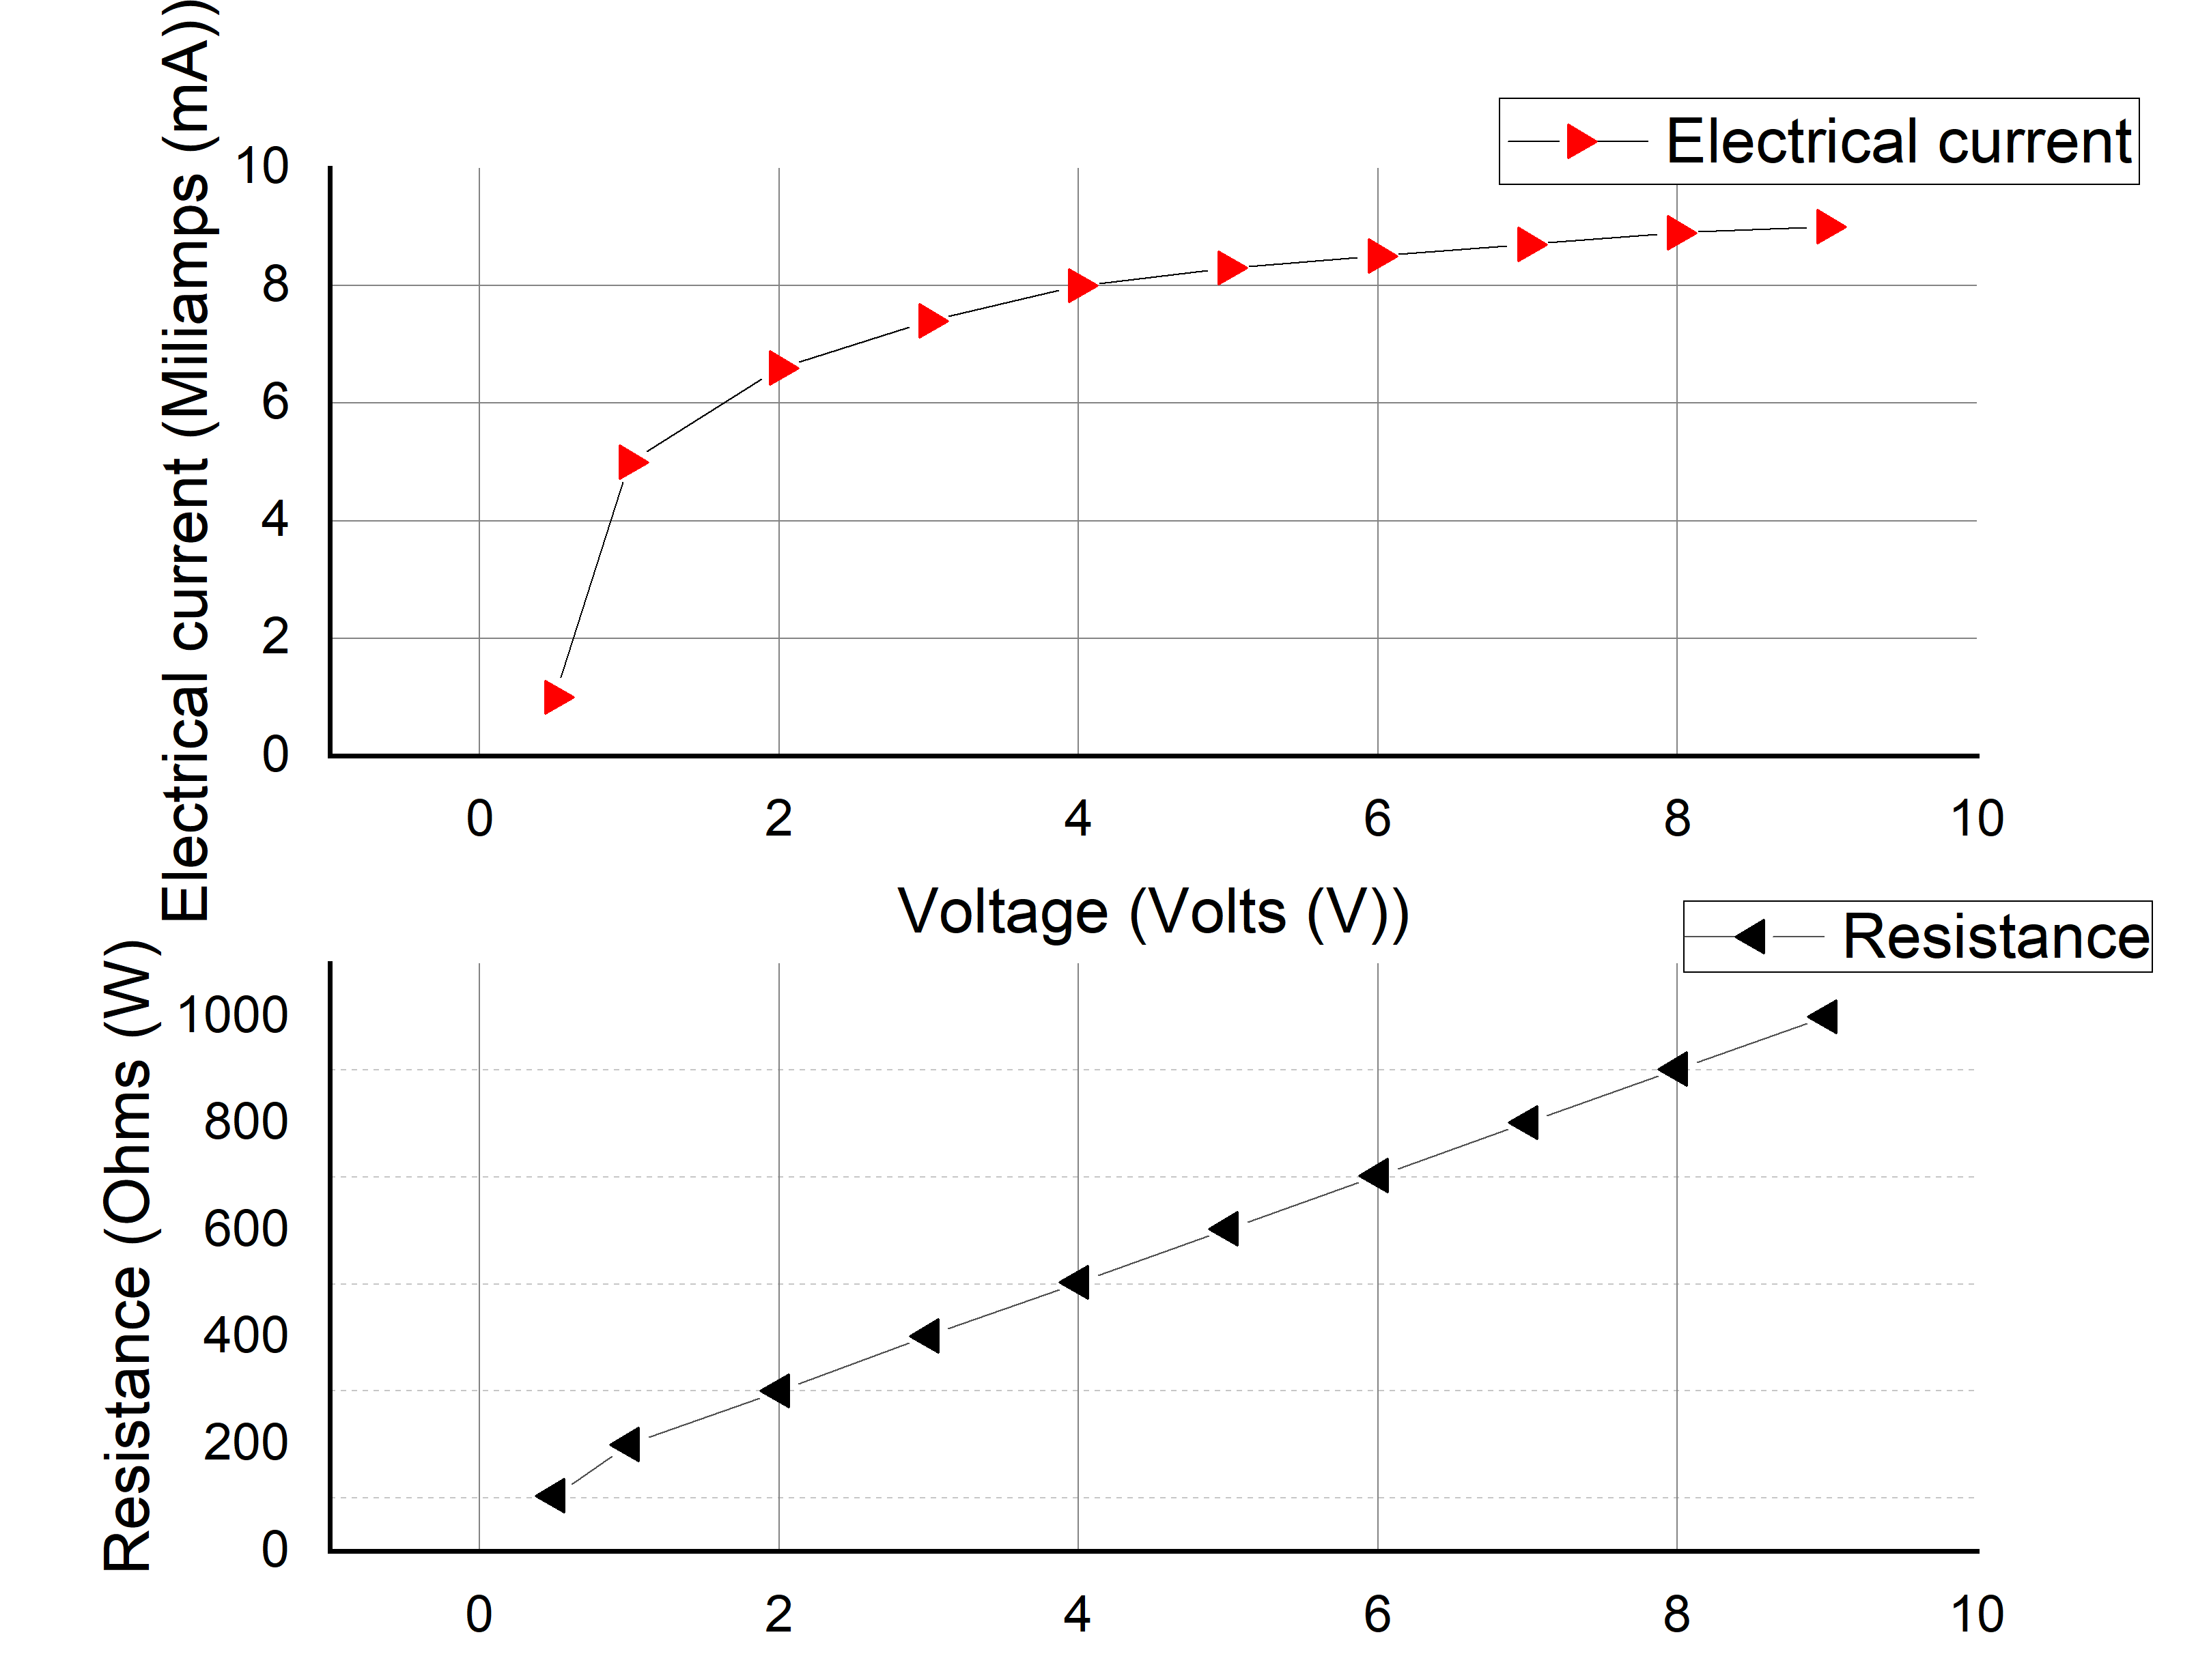
\includegraphics[scale=0.3]{Images/Graph1.png}
      \textcolor{MiColor2}{\textbf{Graph 1:\\ Above: Electric Current where the voltage and the resistance are changing constantly.\\Below: How the voltage and resistance are changing and how this has relation to the graph above.}}
\end{center}
\vspace{2em}
\begin{center}
   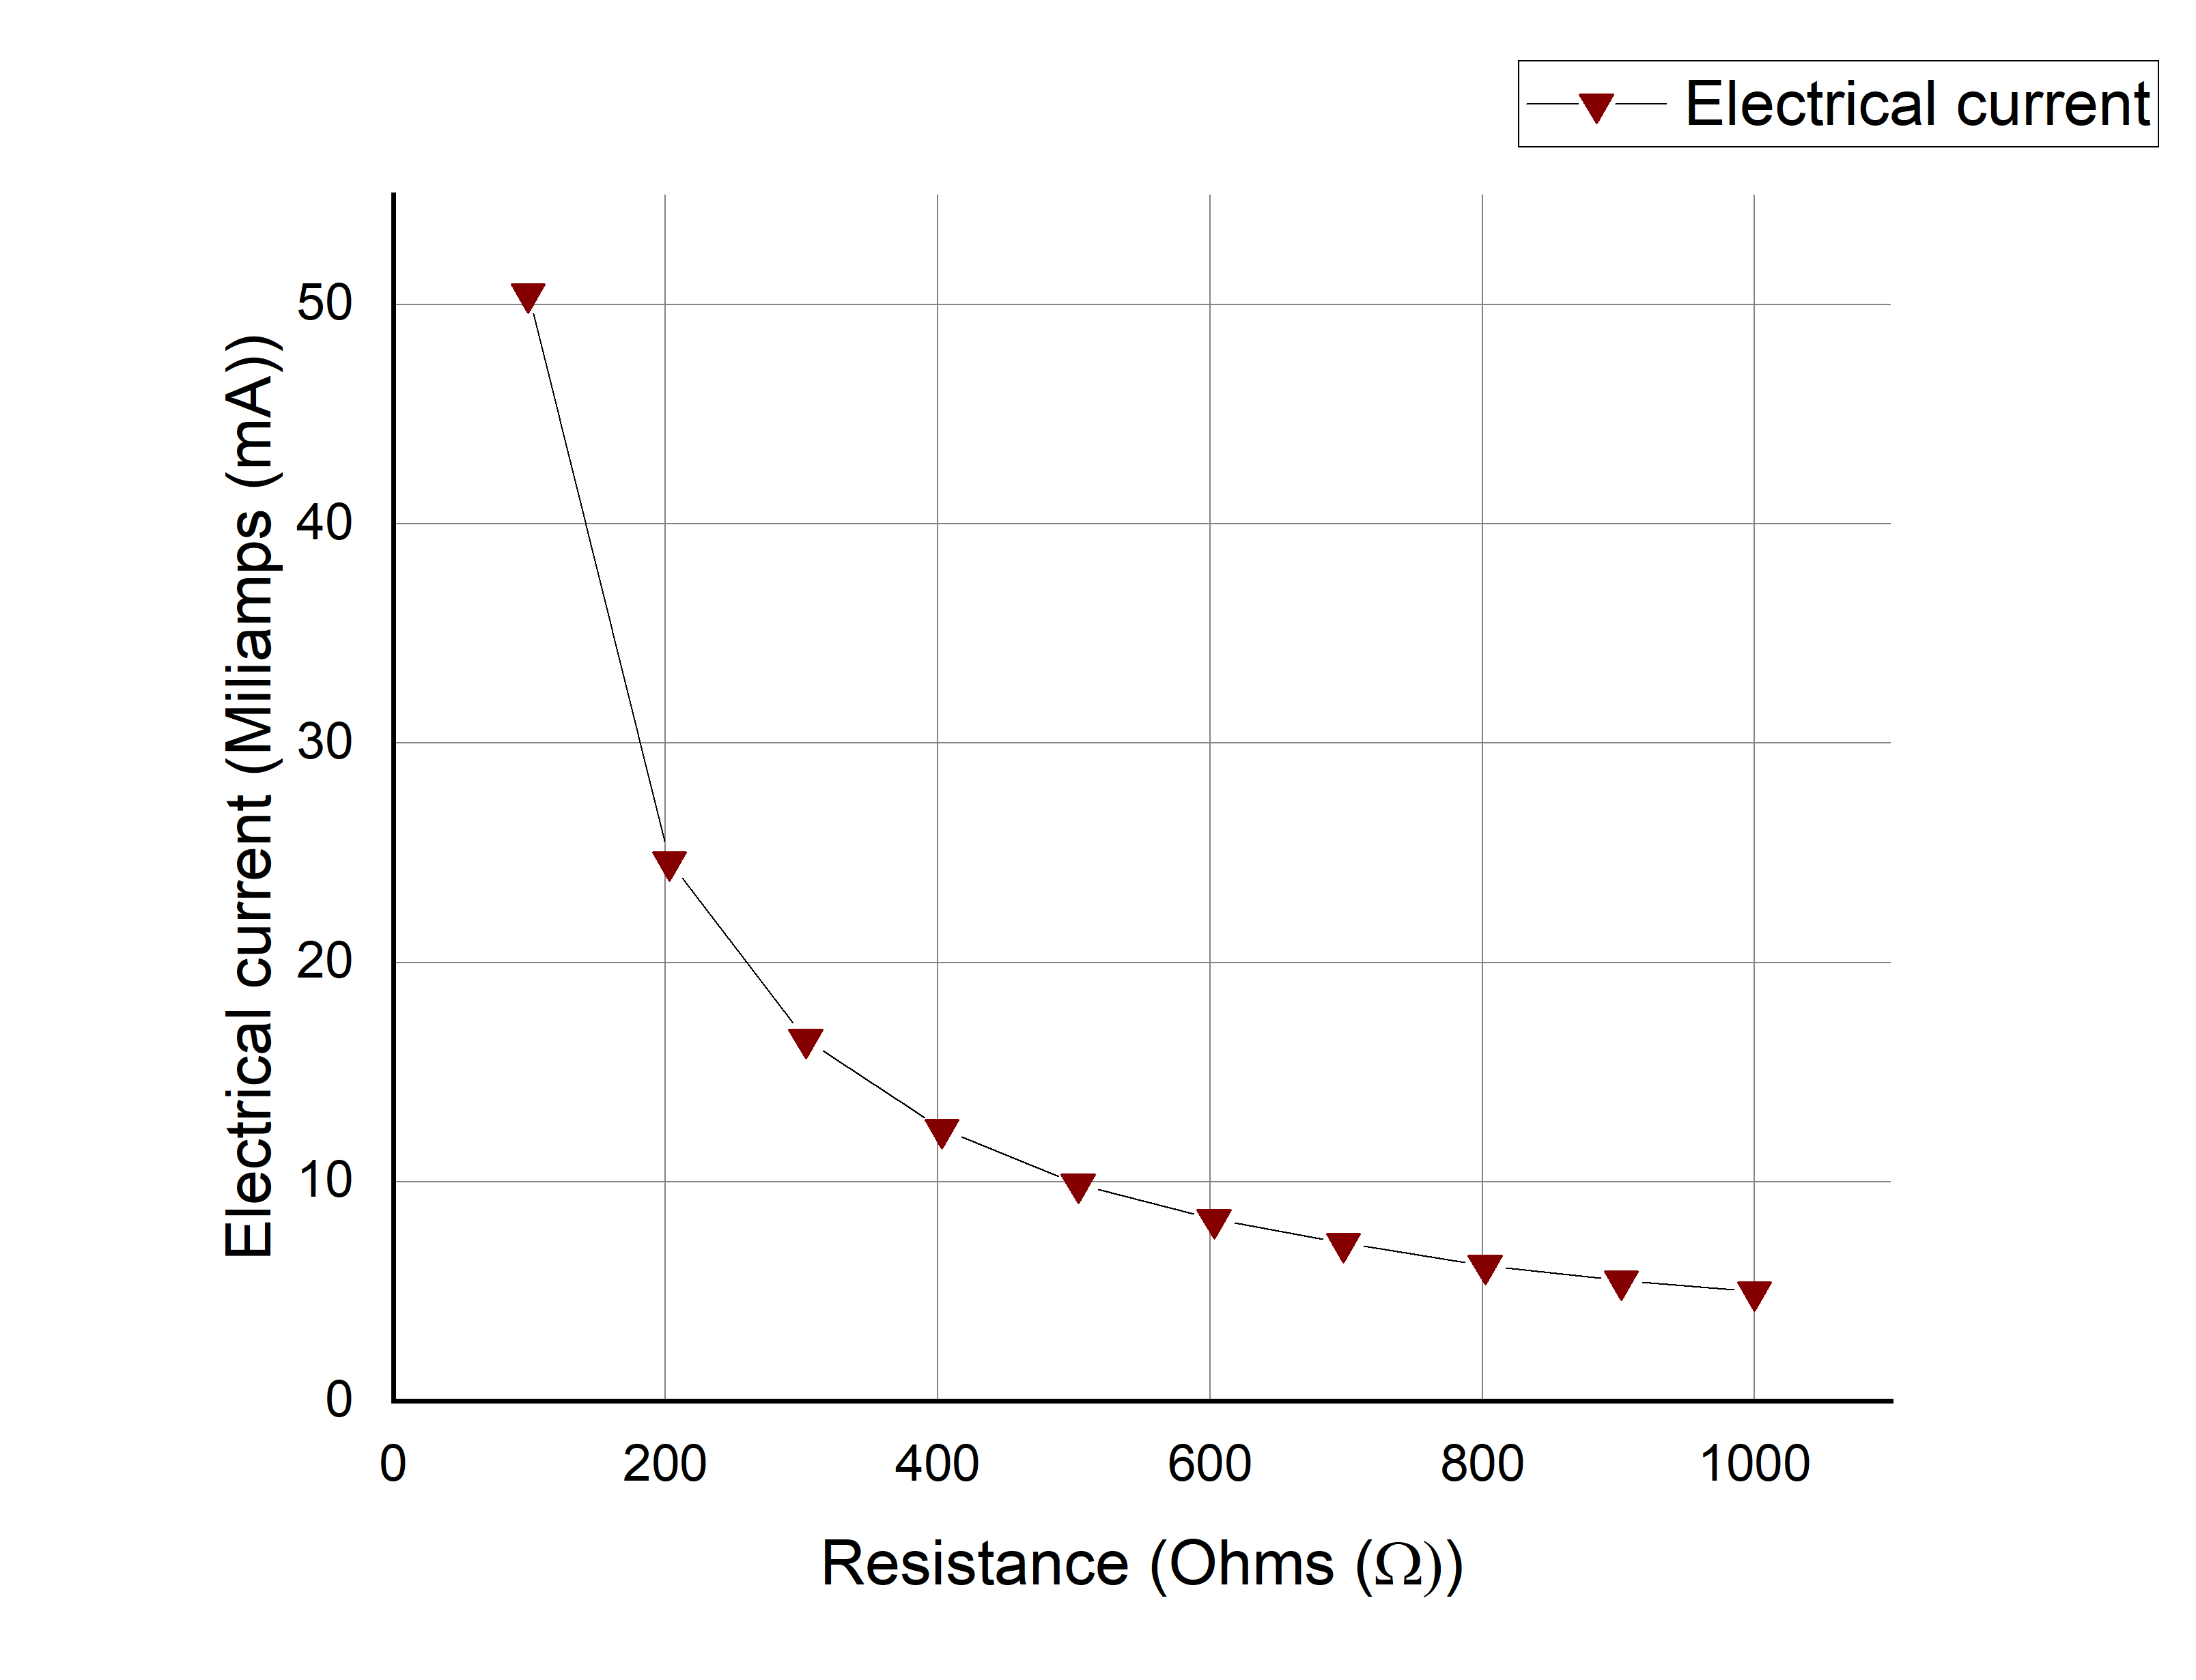
\includegraphics[scale=0.3]{Images/Graph2.png}
    \textcolor{MiColor2}{\textbf{Graph 2: The relation of resistance and electric current when the voltage doesn't changes.}}
\end{center}
\vfill
\newpage

\begin{center}
    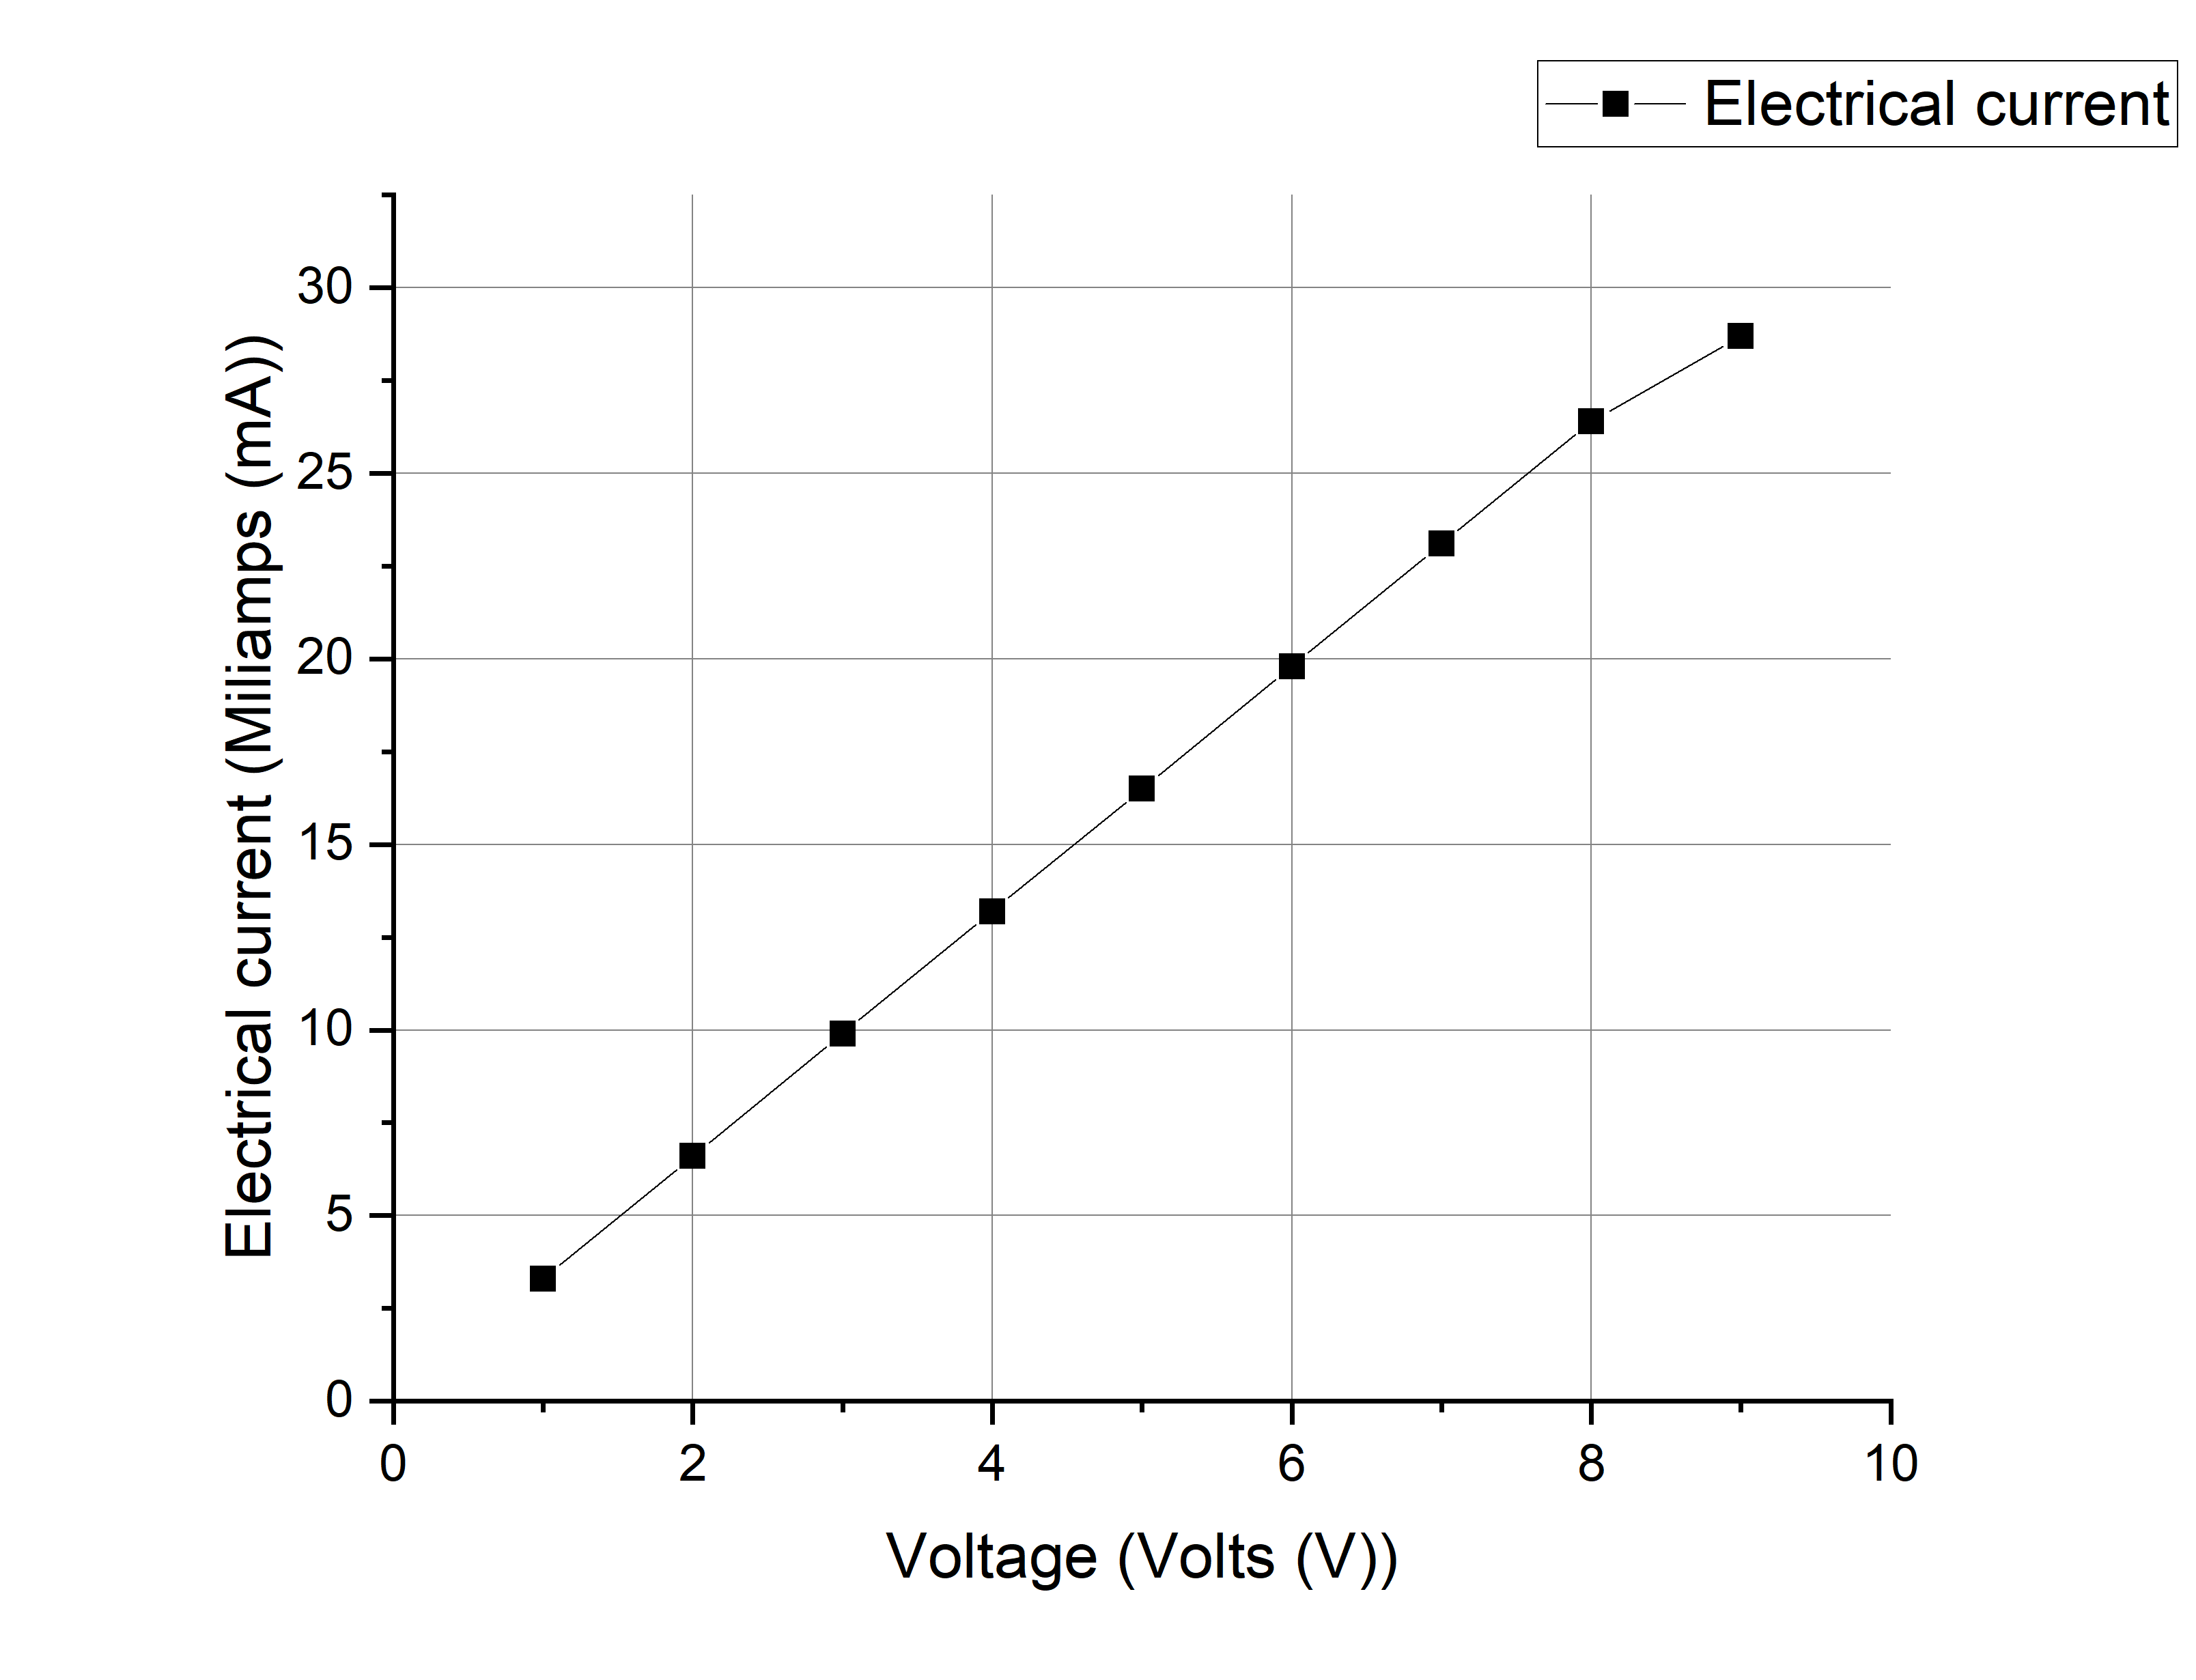
\includegraphics[scale=0.3]{Images/Graph3.png}
    \textcolor{MiColor2}{\textbf{Graph 3: The comportment of electric current and voltage when the resistance doesn't changes.}}
\end{center}



\section{\textcolor{MiColor1}{\textbf{Discussion}}}
Observing the results obtained, in Graph 1:
Above: Electric Current where the voltage and
the resistance are changing constantly.
it was observed a behavior of the graph that looks like an increasing trend with $1 / V ^ 2$.  However, within the degree, a simultaneous constant variation of the voltage is being taken into account along with the resistance with a current at which it remained intact but changing with respect to the other two quantities. Continuing on that same graph, you can see the correspondence of the resistance with the voltage since a linear increasing graph is shown, which indicates that the voltage is linearly proportional to the resistance, as the equations already exposed in the theoretical framework show. And something very similar happens in the following graph Graph 2: The relation of resistance and electric
current when the voltage doesn't change, only aqua if an exponential decay is noted, where the relationship between the intensity and the electrical resistance is linear, which does not quite match the mathematical theory, since in this practice it does not we traffic mistakes. On the other hand in Graph 3: The behavior of electric current
and voltage when the resistance doesn’t
changes, the decay is linear and the slope is negative, which points to this direct proportionality between the voltage corroding.
\section{\textcolor{MiColor1}{\textbf{Conclusions}}}
Throughout this practice, Ohm's law has been verified in the three main senses of mathematical theory. When determining the graphical relationship between voltage (V) and current (I) for a fixed resistance, a line with a positive slope was obtained, which indicates that the two quantities already mentioned are directly proportional to each other. In Graph 2: The relation of resistance and electriccurrent when the voltage doesn’t changes, the results were disconcerting since again a linear behavior was expected, however, an exponential decrease was obtained! With respect to the relationship between resistance and voltage, the two quantities are inversely proportional to each other, concluding in the agreement between the data obtained and the equations.
\section{\textcolor{MiColor1}{\textbf{Acknowledgements}}}
Acknowledgements to Dr. Mario Pérez González for providing us with school support to carry out this practice and knowledge to use the OriginPro software, also an acknowledge all the doctors and experts from the University of Colorado Boulder, because thanks to them we had access to the "PhET" software.

\begin{thebibliography}{}

\bibitem{1}\textcolor{MiColor2}{\protect\href{http://www.labvirfis.com/textos/serway1.pdf}{ R.A. Serway, J.W. Jewett Jr., Física para Ciencias e Ingeniería con Física Moderna, séptima edición, Cengage Learning, México, 2009.}} \par
\bibitem{2}\textcolor{MiColor2}{\protect\href{https://www.u-cursos.cl/usuario/42103e5ee2ce7442a3921d69b0200c93/mi_blog/r/Fisica_General_-_Fisica_Universitaria_Vol_2__ed_12\%28Sears-Zemansky\%29.pdf}{H.D. Young, Y. Freedman, Física Universitaria con Física Moderna, décimo tercera edición, PEARSON, México, 2013.}} \par
\bibitem{3}\textcolor{MiColor2}{\protect\href{http://www.fulviofrisone.com/attachments/article/485/Resnick-Fisica\%20Vol\%202.pdf}{D. Halliday, R. Resnick, \& K.S. Krane, Física Volumen 2, cuarta edición, Editorial Continental, México, 1999.}} \par
\bibitem{4}\textcolor{MiColor2}{\protect\href{https://phet.colorado.edu/sims/html/ohms-law/latest/ohms-law\_en.html}{Ohm's Law. PhET: Interactive Simulations. \\ https://phet.colorado.edu/sims/html/ohms-law/latest/ohms-law\_en.html. \\ 2020 (Accessed 21 August 2020)}} \par
\bibitem{5}\textcolor{Black}{J. Wilson, A.J. Bufa \& B. Lou, Física, Sexta edición, PEARSON, México, 2007.} \par
\bibitem{6}\textcolor{MiColor2}{\protect\href{http://esystems.mx/BPC/llyfrgell/0296.pdf}{D. Giancoli, Física para Ciencias e Ingenierías. Volumen 2, Cuarta edición, PEARSON, México, 2009}}
\bibitem{7}\textcolor{Black}{Stanley V. Marshall, Richard E. DuBroff and Gabriel G. Skitek, Electromagnetismo. Conceptos y Aplicaciones, Cuarta Edición, México, 1997.} \par
\bibitem{8}\textcolor{MiColor2}{\protect\href{http://profesores.dcb.unam.mx/users/raulpm/teoem/griffiths.pdf}{D. Griffiths, Introduction to Electrodynamics, Fourth Edition, PEARSON, United States, 2013.}} \par
\bibitem{9}\textcolor{MiColor2}{\protect\href{https://books.google.com.mx/books?id=GXJ2tfECwV0C\&printsec=frontcover\&hl=es\#v=onepage\&q\&f=false}{U. Bakshi, A. Bakshi, Electrical Circuit Analysis, First Edition, Technical Publications Pune, India, 2008.}}

\end{thebibliography}

\end{multicols}

\end{document}
